\section{Validation, Sensitivity \& Common Pitfalls}

\begin{frame}{Why Validation Matters}
  \begin{itemize}
    \item A model is a \textbf{simplification} of reality --- it is always ``wrong'' in some sense.
    \item The question is: \emph{is the model useful for the intended purpose?}
    \item George Box (1976): \textbf{``All models are wrong, but some are useful.''}
  \end{itemize}
  \medskip
  Three levels of checking:
  \begin{description}
    \item[Verification] Does the code correctly implement the equations?
    \item[Validation] Does the model reproduce observed real-world behaviour?
    \item[Calibration] Can we find parameter values that fit data well?
  \end{description}
\end{frame}

\begin{frame}{Verification: Is the Code Correct?}
  \begin{itemize}
    \item \textbf{Conservation laws}: does $S + I + R = N$ hold at every step?
    \item \textbf{Limiting cases}: does the SIR reduce to exponential decay when $\beta = 0$?
    \item \textbf{Convergence}: does refining $\Delta t$ improve the solution?
    \item \textbf{Comparison}: does the ABM match the ODE for large $N$?
  \end{itemize}
  \begin{center}
    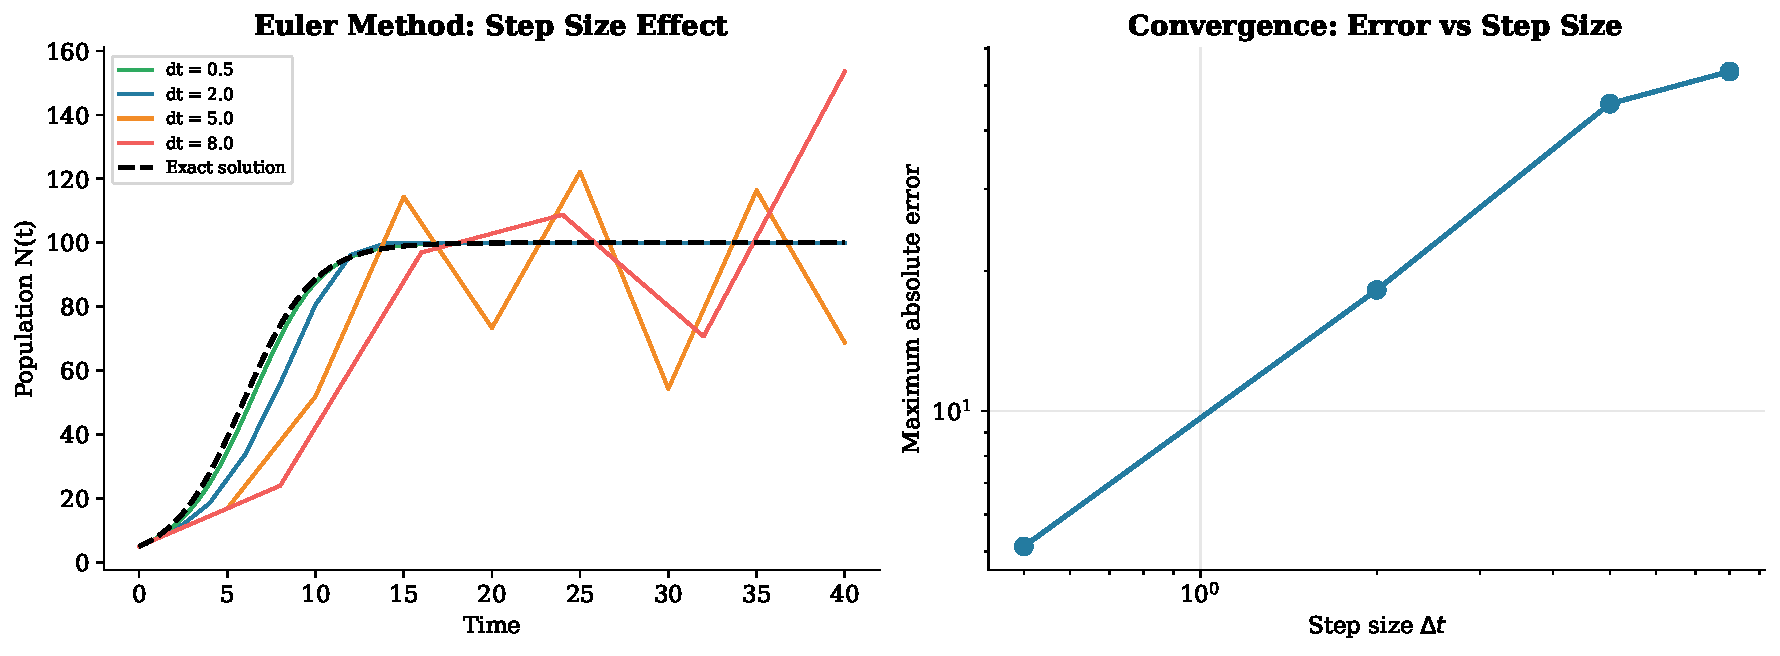
\includegraphics[width=0.85\textwidth]{images/euler_convergence.pdf}
  \end{center}
\end{frame}

\begin{frame}{Validation: Does the Model Match Reality?}
  \begin{itemize}
    \item Compare model output against \textbf{independent data} not used for fitting.
    \item Qualitative: does the model produce the right \emph{shape} of behaviour?
      \begin{itemize}
        \item S-curves, oscillations, extinction thresholds, etc.
      \end{itemize}
    \item Quantitative: compute error metrics ($R^2$, RMSE, AIC).
    \item \textbf{Important}: a model that fits training data perfectly may fail on new data.
  \end{itemize}
\end{frame}

\begin{frame}{The Overfitting Trap}
  \begin{center}
    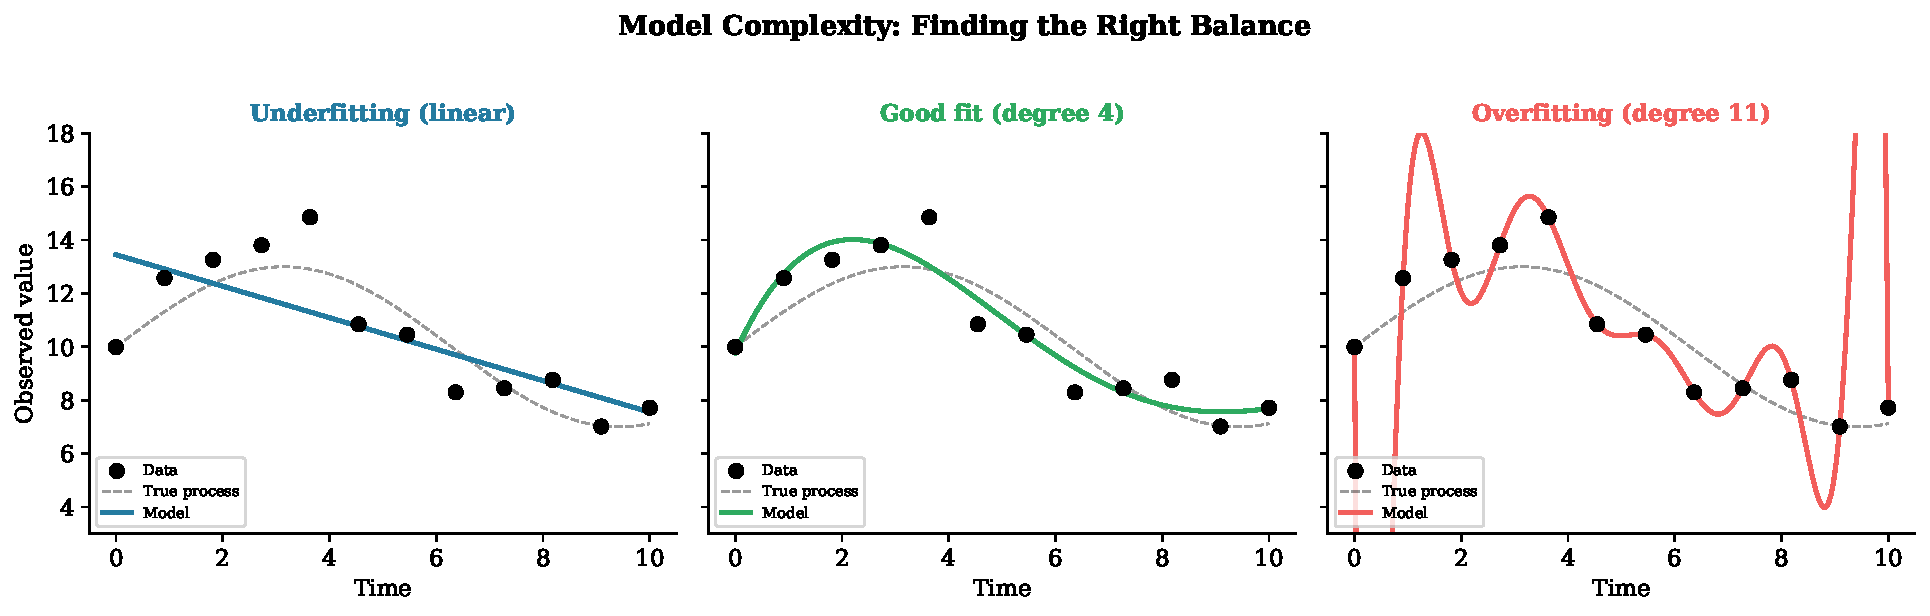
\includegraphics[width=0.95\textwidth]{images/overfitting.pdf}
  \end{center}
  \begin{itemize}
    \item \textbf{Underfitting}: model too simple, misses the pattern.
    \item \textbf{Overfitting}: model too complex, learns the noise.
    \item \textbf{Good fit}: captures the underlying process without chasing noise.
    \item Rule of thumb: \emph{more parameters} $\neq$ \emph{better model}.
  \end{itemize}
\end{frame}

\begin{frame}{Sensitivity Analysis}
  \textbf{Question:} How much does the output change when I vary a parameter?
  \medskip
  \begin{itemize}
    \item Vary one parameter at a time (OAT) while holding others fixed.
    \item Record a key output metric (e.g.\ peak infected, time to extinction).
    \item Visualise with a \textbf{tornado diagram}.
  \end{itemize}
  \begin{center}
    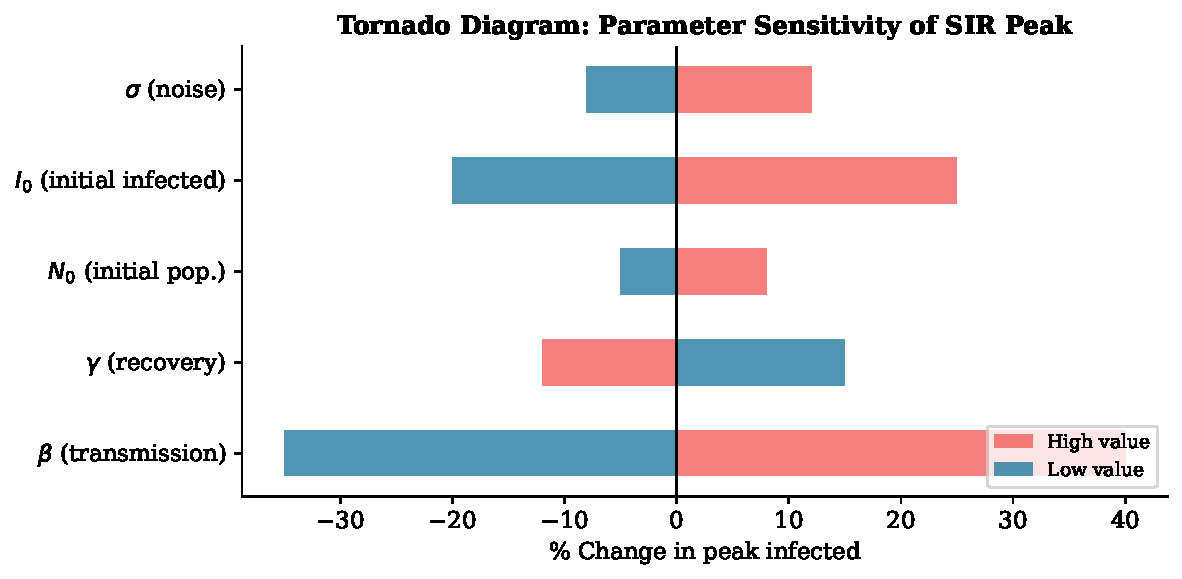
\includegraphics[width=0.72\textwidth]{images/sensitivity_tornado.pdf}
  \end{center}
\end{frame}

\begin{frame}{Sensitivity Analysis: Why It Matters}
  \begin{itemize}
    \item Identifies \textbf{critical parameters} that drive the behaviour.
    \item Reveals which parameters need \textbf{careful measurement} vs.\ rough estimates.
    \item Helps communicate \textbf{uncertainty}: ``If $\beta$ increases by 10\%, the peak doubles.''
    \item For your projects:
    \begin{itemize}
      \item Pick 2--3 key parameters.
      \item Sweep each through a plausible range.
      \item Show how a key output responds.
    \end{itemize}
  \end{itemize}
\end{frame}

\begin{frame}{Common Modelling Pitfalls}
  \begin{enumerate}
    \item \textbf{Ignoring units.} Always track physical units ($\text{time}^{-1}$, individuals, etc.).
    \item \textbf{Step size too large.} Euler's method can diverge or give wrong results.
    \item \textbf{Too many free parameters.} If the model can fit anything, it explains nothing.
    \item \textbf{No baseline comparison.} Always compare against a simpler model or null model.
    \item \textbf{Cherry-picking runs.} In stochastic models, show \emph{ensembles}, not single lucky trajectories.
    \item \textbf{Confusing correlation with causation.} A good fit does not prove the mechanism is correct.
  \end{enumerate}
\end{frame}

\begin{frame}{Stochastic Models: Ensemble Thinking}
  \begin{itemize}
    \item A single ABM run tells you very little --- it is \textbf{one sample} from many possible outcomes.
    \item Always run $N_{\text{runs}} \geq 20$ and report:
    \begin{itemize}
      \item Mean trajectory
      \item Confidence bands (e.g.\ 5th--95th percentile)
      \item Distribution of key outcomes (peak size, final state)
    \end{itemize}
    \item This is not a limitation --- it is a \textbf{feature}: the spread tells you about risk and variability.
  \end{itemize}
\end{frame}
